%%%%%%%%%%%%%%%%%%%%%%%%%%%%%%%%%%%%%%%%%%%%%%%%%%%%%%%%%%%%%%%%%%%%%%%%%%%%%%%%%%
\begin{frame}[fragile]\frametitle{}
\begin{center}
{\Large Fine-tuning LLMs (Large Language Models)}
\end{center}
\end{frame}

%%%%%%%%%%%%%%%%%%%%%%%%%%%%%%%%%%%%%%%%%%%%%%%%%%%%%%%%%%%%%%%%%%%%%%%%%%%%%%%%%%
\begin{frame}[fragile]\frametitle{Introduction to Fine-Tuning}
  \begin{itemize}
    \item \textbf{Definition:} Process of training pre-existing models on smaller, domain-specific datasets to enhance task or domain performance.
    \item \textbf{Objective:} Refine capabilities and adapt models for specific applications.
    \item \textbf{Illustration with GPT-3:}
      \begin{itemize}
        \item GPT-3 designed for diverse NLP tasks but may lack optimization for specific domains.
        \item Example: Healthcare organization fine-tunes GPT-3 for generating patient reports, adapting to medical terminologies.
      \end{itemize}
    \item \textbf{Applicability Beyond LLMs:}
      \begin{itemize}
        \item Not exclusive to language models; applicable to various machine learning models.
        \item Example: Convolutional neural network fine-tuning for detecting trucks on highways.
      \end{itemize}
    \item \textbf{Key Principle:} Leverage pre-trained models, recalibrate parameters using novel data for new contexts or applications.
    \item \textbf{Considerations:} Beneficial when training data distribution significantly differs from specific application requirements.
  \end{itemize}
\end{frame}


%%%%%%%%%%%%%%%%%%%%%%%%%%%%%%%%%%%%%%%%%%%%%%%%%%%%%%%%%%%
\begin{frame}[fragile]\frametitle{What is a fine-tuned LLM?}


		\begin{center}
		\includegraphics[width=\linewidth,keepaspectratio]{rag8}
		\end{center}

{\tiny (Ref: Generative AI with Large Language Model - Abhinav  Kimothi)}

\end{frame}



%%%%%%%%%%%%%%%%%%%%%%%%%%%%%%%%%%%%%%%%%%%%%%%%%%%%%%%%%%%%%%%%%%%%%%%%%%%%%%%%%%
\begin{frame}[fragile]\frametitle{Why Fine-Tuning?}
  \begin{itemize}
    \item \textbf{General Models vs. Specialization:}
      \begin{itemize}
        \item Large language models designed for versatility, not task mastery.
        \item Fine-tuning essential for exceptional proficiency in specific tasks or domains.
      \end{itemize}
    \item \textbf{Versatility vs. Mastery:}
      \begin{itemize}
        \item Generic models proficient in multiple tasks but lack mastery.
        \item Fine-tuned models optimized for specific tasks, achieving mastery.
      \end{itemize}
    \item \textbf{Decision to Fine-Tune:}
      \begin{itemize}
        \item Driven by the need for superior performance in targeted applications.
        \item Highly effective specialists in designated areas.
      \end{itemize}
  \end{itemize}
\end{frame}


%%%%%%%%%%%%%%%%%%%%%%%%%%%%%%%%%%%%%%%%%%%%%%%%%%%%%%%%%%%%%%%%%%%%%%%%%%%%%%%%%%
\begin{frame}[fragile]\frametitle{Why Fine-Tuning?}
    \begin{itemize}
        \item Pre-trained models are trained and built with general-purpose tasks, with Fine-tuning we can improve the performance of pre-trained models in wide range of domain-specific tasks.
        \item Fine-tuning is a technique where a pre-trained model is trained on a new dataset.
		\item Fine Tuning has many approaches, one uses adjusting last layer with retraining on custom data, another has adopter auxiliary network which gets trained on custom data, some have full retraining with frozen earlier weights.
		\item Fine-tuning leverages a pre-trained model's knowledge and capabilities, saving significant time and resources compared to training a model from scratch. 
		\item Improve factual response by utilizing Domain-specific data. 
		\item Reduce Hallucinations.
    \end{itemize}
\end{frame}

%%%%%%%%%%%%%%%%%%%%%%%%%%%%%%%%%%%%%%%%%%%%%%%%%%%%%%%%%%%
\begin{frame}[fragile]\frametitle{What is a fine-tuned LLM?}

\begin{itemize}
  \item \textbf{Context Learning Limitation:}
    \begin{itemize}
      \item Through in-context learning or prompting, only a limited performance level is achievable.
    \end{itemize}

  \item \textbf{Challenges of Few-Shot Learning:}
    \begin{itemize}
      \item Few-shot learning may not be effective for smaller LLMs.
      \item Consumes significant space in the context window.
    \end{itemize}

  \item \textbf{Fine Tuning Overview:}
    \begin{itemize}
      \item Supervised learning process adjusting LLM weights.
      \item Uses a labeled dataset of prompt-completion pairs.
    \end{itemize}

  \item \textbf{Instruction Fine Tuning:}
    \begin{itemize}
      \item Trains LLM on examples of instructions and desired responses.
      \item Improves performance on instruction-specific tasks.
    \end{itemize}

  \item \textbf{Full Fine Tuning:}
    \begin{itemize}
      \item Updates all LLM parameters.
      \item Requires sufficient memory for storing and processing gradients and components.
    \end{itemize}
\end{itemize}


{\tiny (Ref: Generative AI with Large Language Model - Abhinav  Kimothi)}

\end{frame}


%%%%%%%%%%%%%%%%%%%%%%%%%%%%%%%%%%%%%%%%%%%%%%%%%%%%%%%%%%%%%%%%%%%%%%%%%%%%%%%%%%
\begin{frame}[fragile]\frametitle{Reasons for Fine-Tuning - Part 1}
  \begin{itemize}
    \item \textbf{Domain-Specific Adaptation:}
      \begin{itemize}
        \item Pre-trained LLMs not optimized for specific tasks or domains.
        \item Fine-tuning allows adaptation to nuances, enhancing performance.
        \item Example: Fine-tuning for document analysis in the legal domain.
      \end{itemize}
    \item \textbf{Shifts in Data Distribution:}
      \begin{itemize}
        \item Models may not generalize well to out-of-distribution examples.
        \item Fine-tuning aligns the model with new data distribution, improving performance.
        \item Example: Fine-tuning a sentiment analysis model for social media comments.
      \end{itemize}
    \item \textbf{Cost and Resource Efficiency:}
      \begin{itemize}
        \item Training from scratch requires a large dataset, fine-tuning is more efficient.
        \item Example: Adapting a pre-trained model for small e-commerce platform recommendations.
      \end{itemize}
  \end{itemize}
\end{frame}

%%%%%%%%%%%%%%%%%%%%%%%%%%%%%%%%%%%%%%%%%%%%%%%%%%%%%%%%%%%%%%%%%%%%%%%%%%%%%%%%%%
\begin{frame}[fragile]\frametitle{Reasons for Fine-Tuning - Part 2}
  \begin{itemize}
    \item \textbf{Out-of-Distribution Data Handling:}
      \begin{itemize}
        \item Fine-tuning mitigates suboptimal performance with modest dataset.
        \item Example: Fine-tuning a speech recognition model for a new regional accent.
      \end{itemize}
    \item \textbf{Knowledge Transfer:}
      \begin{itemize}
        \item Fine-tuning transfers general knowledge from pre-trained models to specific tasks.
        \item Example: Transferring medical knowledge to a healthcare chatbot.
      \end{itemize}
    \item \textbf{Task-Specific Optimization:}
      \begin{itemize}
        \item Fine-tuning optimizes model parameters for specific task objectives.
        \item Example: Optimizing a pre-trained model for code generation in software development.
      \end{itemize}
  \end{itemize}
\end{frame}


%%%%%%%%%%%%%%%%%%%%%%%%%%%%%%%%%%%%%%%%%%%%%%%%%%%%%%%%%%%%%%%%%%%%%%%%%%%%%%%%%%
\begin{frame}[fragile]\frametitle{Reasons for Fine-Tuning - Part 3}
  \begin{itemize}
    \item \textbf{Adaptation to User Preferences:}
      \begin{itemize}
        \item Fine-tuning aligns the model with user preferences and task requirements.
        \item Example: Fine-tuning a virtual assistant model for user-specific language and tone.
      \end{itemize}
    \item \textbf{Continual Learning:}
      \begin{itemize}
        \item Fine-tuning supports continual learning, adapting to evolving data and user needs.
        \item Example: Continually updating a news summarization model for evolving news topics.
      \end{itemize}
  \end{itemize}
\end{frame}

%%%%%%%%%%%%%%%%%%%%%%%%%%%%%%%%%%%%%%%%%%%%%%%%%%%%%%%%%%%%%%%%%%%%%%%%%%%%%%%%%%
\begin{frame}[fragile]\frametitle{Challenges and Solutions: In-Context Learning}
    \begin{itemize}
        \item Prominent technique for task-specific adaptation.
        \item Challenges include limited context window and real-time optimization.
        \item Context window restricts processing of long sequences.
        \item Real-time optimization is difficult during progression through the context window.
    \end{itemize}
\end{frame}

%%%%%%%%%%%%%%%%%%%%%%%%%%%%%%%%%%%%%%%%%%%%%%%%%%%%%%%%%%%%%%%%%%%%%%%%%%%%%%%%%%
\begin{frame}[fragile]\frametitle{Challenges with Few-Shot Learning}
    \begin{itemize}
        \item Effective for larger LLMs, less so for smaller models.
        \item Smaller models struggle to learn complex patterns from few examples.
        \item Few-shot learning demands a large context window.
        \item Resource-intensive and impractical for memory-constrained environments.
    \end{itemize}
\end{frame}

%%%%%%%%%%%%%%%%%%%%%%%%%%%%%%%%%%%%%%%%%%%%%%%%%%%%%%%%%%%%%%%%%%%%%%%%%%%%%%%%%%
\begin{frame}[fragile]\frametitle{Understanding Fine-Tuning}
    \begin{itemize}
        \item Widely used for customizing pre-trained LLMs to specific tasks.
        \item Involves training on labeled prompt-completion pairs.
        \item Allows model to adjust weights for task alignment.
    \end{itemize}
\end{frame}

%%%%%%%%%%%%%%%%%%%%%%%%%%%%%%%%%%%%%%%%%%%%%%%%%%%%%%%%%%%%%%%%%%%%%%%%%%%%%%%%%%
\begin{frame}[fragile]\frametitle{Unsupervised Fine-Tuning Methods}

\begin{itemize}
\item \textbf{Unsupervised Full Fine-Tuning:}
  \begin{itemize}
	\item Relevant for updating LLM knowledge base without changing existing behavior.
	\item Example: Fine-tuning on legal literature or adapting to a new language using unstructured datasets.
  \end{itemize}
\item \textbf{Contrastive Learning:}
  \begin{itemize}
	\item Trains the model to discern between similar and dissimilar examples in the latent space.
	\item Beneficial for tasks requiring nuanced understanding of similarities and distinctions.
  \end{itemize}
\end{itemize}
\end{frame}

%%%%%%%%%%%%%%%%%%%%%%%%%%%%%%%%%%%%%%%%%%%%%%%%%%%%%%%%%%%%%%%%%%%%%%%%%%%%%%%%%%
\begin{frame}[fragile]\frametitle{Supervised Fine-Tuning Methods}

\begin{itemize}
\item \textbf{Parameter-Efficient Fine-Tuning (PEFT):}
  \begin{itemize}
	\item Aims to reduce computational expenses by selectively updating a small set of parameters.
	\item Example: Low-rank adaptation (LoRA) technique focuses on updating only relevant parameters.
  \end{itemize}
\item \textbf{Supervised Full Fine-Tuning:}
  \begin{itemize}
	\item Involves updating all parameters of the language model during training.
	\item Resource-intensive but ensures thorough adaptation of the entire model to the task or domain.
  \end{itemize}
\item \textbf{Instruction Fine-Tuning:}
  \begin{itemize}
	\item Involves training the model using examples with explicit instructions for specific queries or tasks.
	\item Suitable for applications where precise task execution is essential.
  \end{itemize}
\item \textbf{Reinforcement Learning from Human Feedback (RLHF):}
  \begin{itemize}
	\item Incorporates reinforcement learning principles with human evaluators providing ratings.
	\item Ratings serve as rewards, guiding the model to optimize parameters based on human preferences.
  \end{itemize}
\end{itemize}

\end{frame}

%%%%%%%%%%%%%%%%%%%%%%%%%%%%%%%%%%%%%%%%%%%%%%%%%%%%%%%%%%%%%%%%%%%%%%%%%%%%%%%%%%
\begin{frame}[fragile]\frametitle{Instruction Fine-Tuning}
  \begin{itemize}
    \item \textbf{Overview:}
      \begin{itemize}
        \item Instruction fine-tuning enhances LLMs for real-world applications.
        \item Differs from standard supervised fine-tuning by augmenting examples with explicit instructions.
        \item Instruction-tuned models generalize effectively to new tasks, providing additional context.
      \end{itemize}
    \item \textbf{Value in NLP and ML:}
      \begin{itemize}
        \item Instruction fine-tuning is crucial in the evolving landscape of NLP and ML.
        \item Enables LLMs to adapt to specific tasks with nuanced instructions.
      \end{itemize}	  
  \end{itemize}

\begin{center}
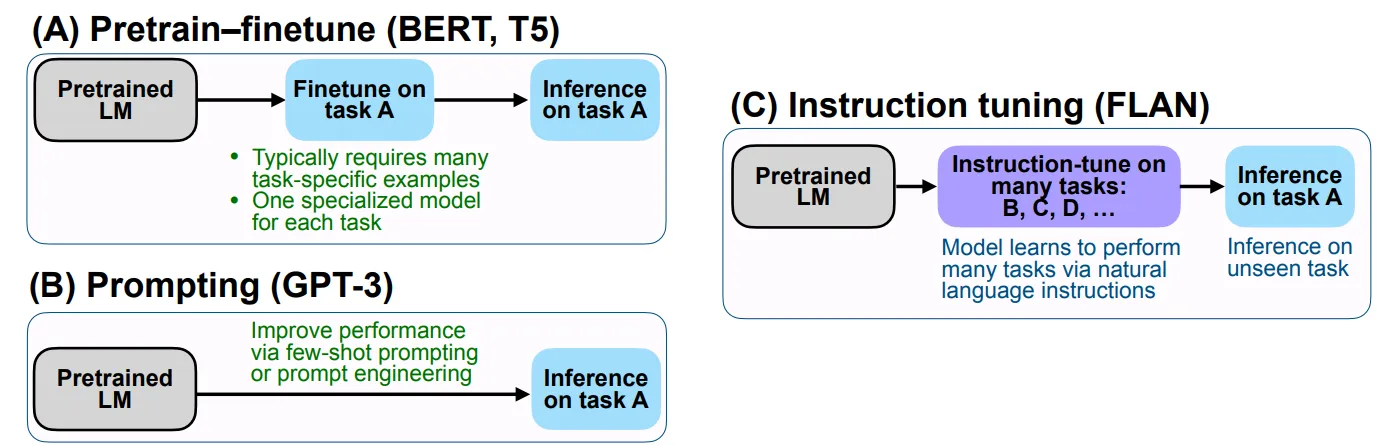
\includegraphics[width=\linewidth,keepaspectratio]{llm128}
\end{center}				

{\tiny (Ref: Applied LLMs Mastery 2024 - Aishwarya Reganti)}

\end{frame}


%%%%%%%%%%%%%%%%%%%%%%%%%%%%%%%%%%%%%%%%%%%%%%%%%%%%%%%%%%%%%%%%%%%%%%%%%%%%%%%%%%
\begin{frame}[fragile]\frametitle{Natural Instructions Dataset}
  \begin{itemize}
    \item \textbf{Dataset Overview:}
      \begin{itemize}
        \item "Natural Instructions" dataset consists of 193,000 instruction-output examples.
        \item Sourced from 61 existing English NLP tasks.
        \item Structured approach with crowd-sourced instructions aligned to a common schema.
      \end{itemize}
    \item \textbf{Unique Features:}
      \begin{itemize}
        \item Each instruction associated with a task, providing explicit guidance for the model.
        \item Covers fields like definition, things to avoid, positive and negative examples.
        \item Structured nature makes it valuable for fine-tuning, offering clear and detailed instructions.
      \end{itemize}
  \end{itemize}
\end{frame}


%%%%%%%%%%%%%%%%%%%%%%%%%%%%%%%%%%%%%%%%%%%%%%%%%%%%%%%%%%%%%%%%%%%%%%%%%%%%%%%%%%
\begin{frame}[fragile]\frametitle{Natural Instructions Example}

\begin{center}
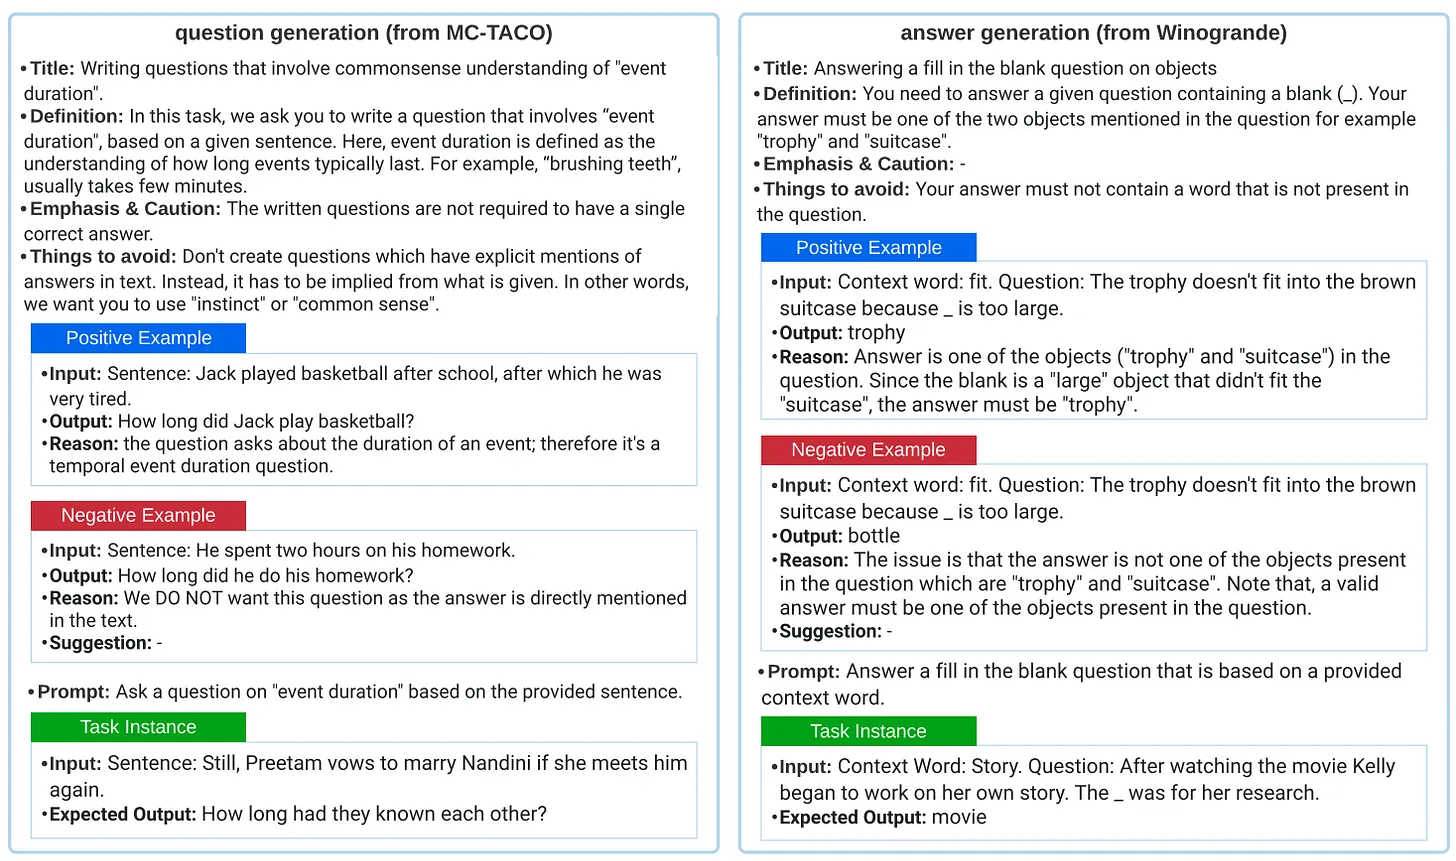
\includegraphics[width=\linewidth,keepaspectratio]{llm129}
\end{center}				

{\tiny (Ref: Applied LLMs Mastery 2024 - Aishwarya Reganti)}

\end{frame}

%%%%%%%%%%%%%%%%%%%%%%%%%%%%%%%%%%%%%%%%%%%%%%%%%%%%%%%%%%%%%%%%%%%%%%%%%%%%%%%%%%
\begin{frame}[fragile]\frametitle{Leveraging Instruction Fine-Tuning}
    \begin{itemize}
        \item Extension of traditional fine-tuning.
        \item Trains model on examples of instructions and desired responses.
        \item Offers improved interpretability, controlled outputs, and reduced biases.
        \item Enables explicit task specification learning for enhanced performance.
    \end{itemize}
\end{frame}

%%%%%%%%%%%%%%%%%%%%%%%%%%%%%%%%%%%%%%%%%%%%%%%%%%%%%%%%%%%%%%%%%%%%%%%%%%%%%%%%%%
\begin{frame}[fragile]\frametitle{Full Fine-Tuning Potential}
    \begin{itemize}
        \item Updates all parameters of the language model during training.
        \item Enhances adaptability to specific tasks for potentially better performance.
        \item Demands significant memory for processing gradients and other components.
        \item Challenging to implement on resource-constrained devices or environments.
    \end{itemize}
\end{frame}

%%%%%%%%%%%%%%%%%%%%%%%%%%%%%%%%%%%%%%%%%%%%%%%%%%%%%%%%%%%%%%%%%%%%%%%%%%%%%%%%%%
\begin{frame}[fragile]\frametitle{Reinforcement Learning from Human Feedback (RLHF)}
  \begin{itemize}
    \item \textbf{Overview:}
      \begin{itemize}
        \item RLHF enhances language models by incorporating human feedback.
        \item Aims to align models more closely with intricate human values.
      \end{itemize}
  \end{itemize}
  
\begin{center}
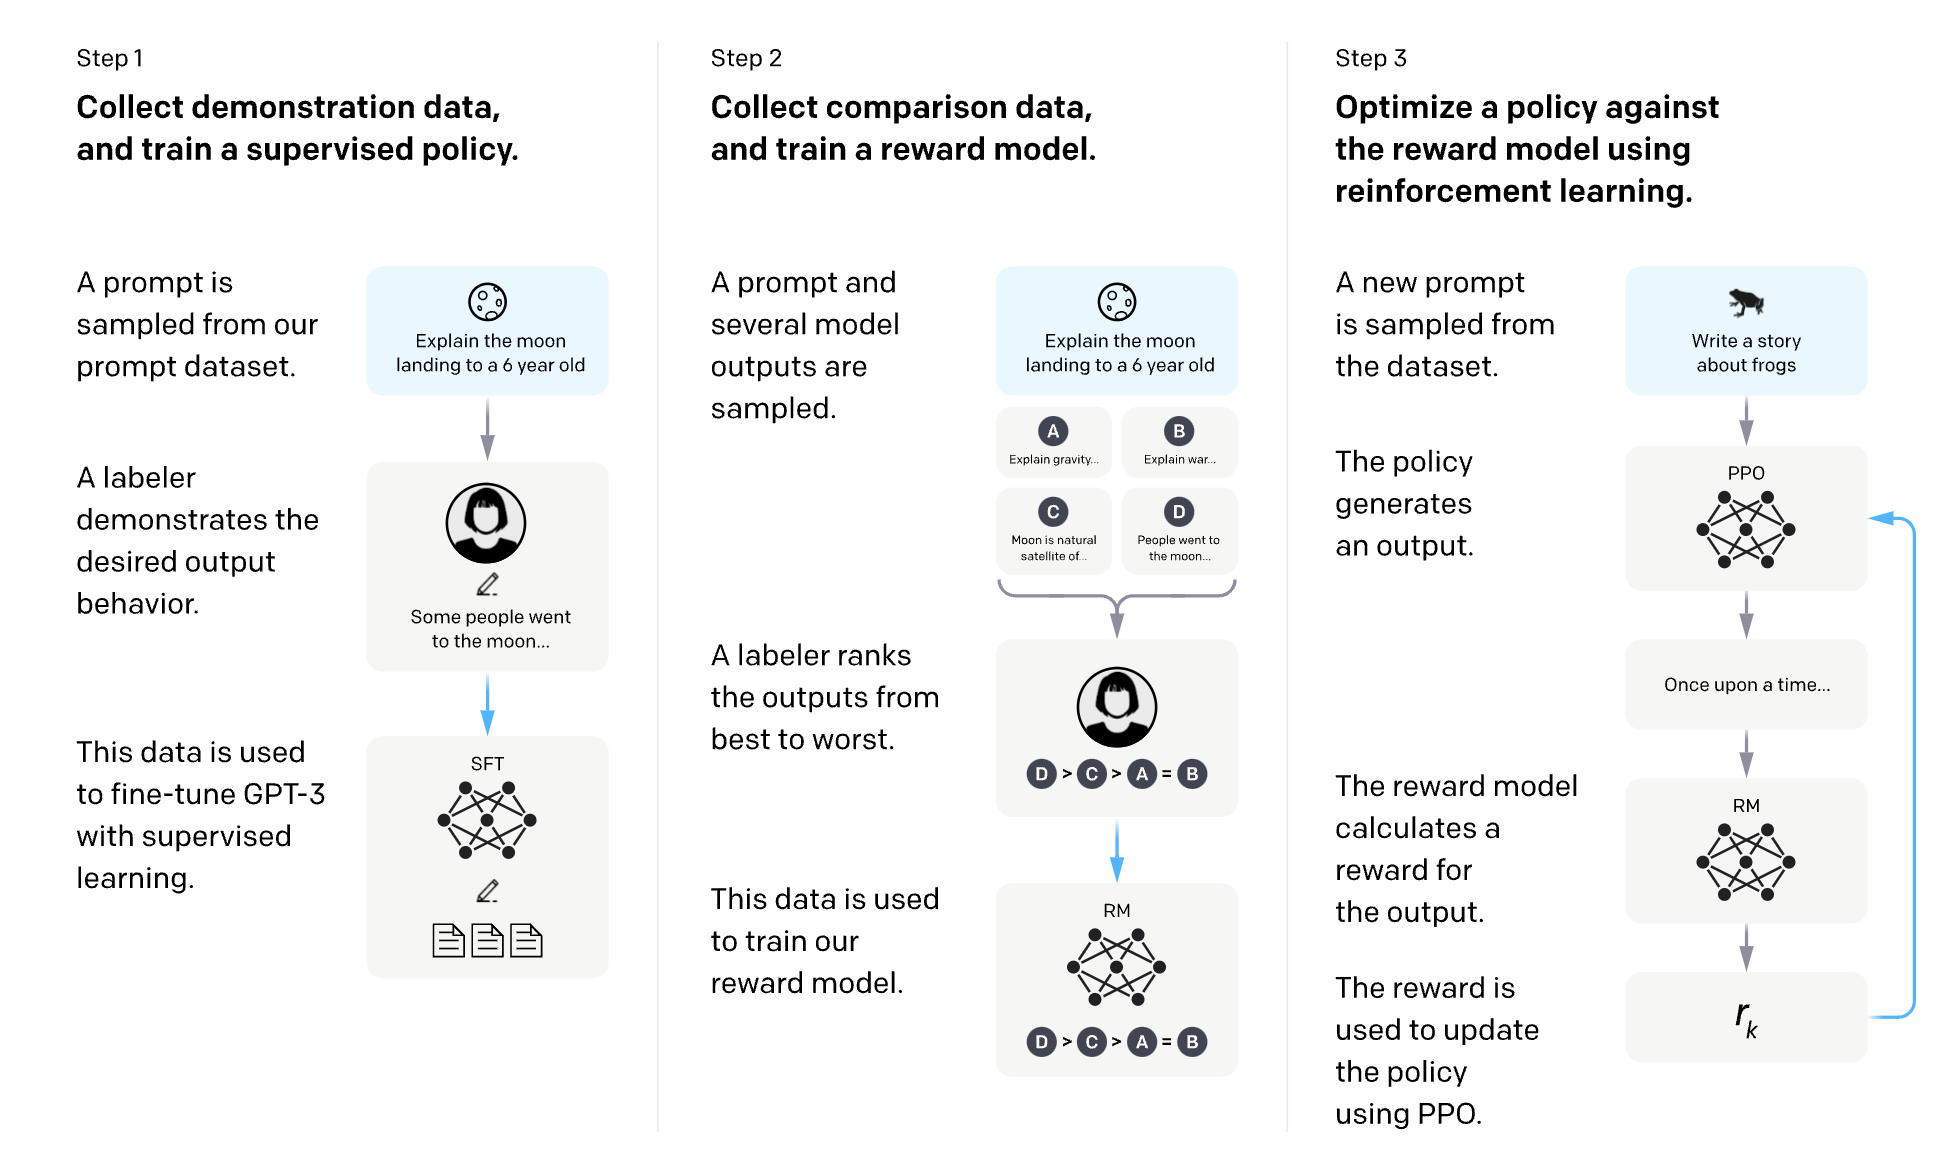
\includegraphics[width=0.8\linewidth,keepaspectratio]{llm130}
\end{center}				

{\tiny (Ref: Applied LLMs Mastery 2024 - Aishwarya Reganti)}  
\end{frame}

%%%%%%%%%%%%%%%%%%%%%%%%%%%%%%%%%%%%%%%%%%%%%%%%%%%%%%%%%%%%%%%%%%%%%%%%%%%%%%%%%%
\begin{frame}[fragile]\frametitle{RLHF Process - Step 1}
  \begin{itemize}
    \item \textbf{Pretraining Language Models (LMs):}
      \begin{itemize}
        \item RLHF starts with a pretrained LM, typically achieved through classical pretraining objectives.
        \item Initial LM, flexible in size, can undergo optional fine-tuning on additional data.
        \item Crucial to have a model with positive response to diverse instructions.
      \end{itemize}
  \end{itemize}
\end{frame}

%%%%%%%%%%%%%%%%%%%%%%%%%%%%%%%%%%%%%%%%%%%%%%%%%%%%%%%%%%%%%%%%%%%%%%%%%%%%%%%%%%
\begin{frame}[fragile]\frametitle{RLHF Process - Step 2}
  \begin{itemize}
    \item \textbf{Reward Model Training:}
      \begin{itemize}
        \item Involves generating a reward model (RM) calibrated with human preferences.
        \item RM assigns scalar rewards to text sequences, reflecting human preferences.
        \item Dataset for training RM generated by sampling prompts, passing through initial LM, and ranking by human annotators.
        \item Reward function combines preference model and a penalty on RL policy vs. initial model difference.
      \end{itemize}
  \end{itemize}
\end{frame}

%%%%%%%%%%%%%%%%%%%%%%%%%%%%%%%%%%%%%%%%%%%%%%%%%%%%%%%%%%%%%%%%%%%%%%%%%%%%%%%%%%
\begin{frame}[fragile]\frametitle{RLHF Process - Step 3}
  \begin{itemize}
    \item \textbf{Fine-Tuning with RL:}
      \begin{itemize}
        \item Final step involves fine-tuning the initial LLM using reinforcement learning.
        \item Proximal Policy Optimization (PPO) commonly used for RL algorithm.
        \item RL policy is LM that takes prompt, produces text, with actions corresponding to tokens in LM's vocabulary.
        \item PPO updates LM's parameters to maximize reward metrics, aligning model with human preferences.
        \item Some parameters frozen due to computational constraints.
      \end{itemize}
  \end{itemize}
\end{frame}

%%%%%%%%%%%%%%%%%%%%%%%%%%%%%%%%%%%%%%%%%%%%%%%%%%%%%%%%%%%%%%%%%%%%%%%%%%%%%%%%%%
\begin{frame}[fragile]\frametitle{Direct Preference Optimization (DPO)}
  \begin{itemize}
    \item \textbf{Overview:}
      \begin{itemize}
        \item DPO is equivalent to RLHF and gaining significant traction.
        \item Offers a straightforward method for fine-tuning large language models based on human preferences.
        \item Eliminates the need for a complex reward model, directly incorporating user feedback into the optimization process.
      \end{itemize}
    \item \textbf{User-Friendly Approach:}
      \begin{itemize}
        \item Users compare two model-generated outputs and express preferences.
        \item LLM adjusts its behavior accordingly, simplifying the optimization process.
        \item Advantages include ease of implementation, computational efficiency, and greater control over LLM's behavior.
      \end{itemize}
  \end{itemize}

\begin{center}
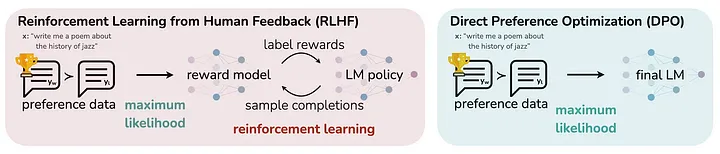
\includegraphics[width=\linewidth,keepaspectratio]{llm131}
\end{center}				

{\tiny (Ref: Applied LLMs Mastery 2024 - Aishwarya Reganti)}

\end{frame}


%%%%%%%%%%%%%%%%%%%%%%%%%%%%%%%%%%%%%%%%%%%%%%%%%%%%%%%%%%%%%%%%%%%%%%%%%%%%%%%%%%
\begin{frame}[fragile]\frametitle{Comparison: DPO vs RLHF}
  \begin{itemize}
    \item \textbf{DPO Approach:}
      \begin{itemize}
        \item Directly optimizes LM based on user preferences without a separate reward model.
        \item Users compare two model-generated outputs to guide the optimization process.
      \end{itemize}

    \item \textbf{Maximum Likelihood in LLM Training:}
      \begin{itemize}
        \item Maximum likelihood is a principle used during LLM training.
        \item Involves adjusting model's parameters to maximize the likelihood of generating actual sequences observed in training data.
        \item Helps LLM learn to generate text similar to examples it was trained on.
      \end{itemize}
    \item \textbf{RLHF Approach:}
      \begin{itemize}
        \item Follows a more structured path, leveraging reinforcement learning principles.
        \item Involves training a reward model to identify and reward desirable LM outputs.
        \item Reward model guides LM's training process, shaping its behavior towards positive outcomes.
      \end{itemize}
    \item \textbf{DPO - A Simpler Approach:}
      \begin{itemize}
        \item Direct Policy Optimization (DPO) takes a straightforward path.
        \item Sidesteps the need for a complex reward model in fine-tuning Large Language Models (LLMs).
        \item Optimizes LLM directly based on user preferences by comparing two outputs.
      \end{itemize}
  \end{itemize}
\end{frame}

%%%%%%%%%%%%%%%%%%%%%%%%%%%%%%%%%%%%%%%%%%%%%%%%%%%%%%%%%%%%%%%%%%%%%%%%%%%%%%%%%%
\begin{frame}[fragile]\frametitle{DPO Advantages}
  \begin{itemize}
    \item \textbf{Ease of Implementation:}
      \begin{itemize}
        \item DPO is more user-friendly, eliminating the need for a separate reward model.
        \item Accessible to a broader audience due to its simplicity.
      \end{itemize}
    \item \textbf{Computational Efficiency:}
      \begin{itemize}
        \item Operates directly on the LLM, leading to faster training times.
        \item Lower computational costs compared to RLHF.
      \end{itemize}
    \item \textbf{Greater Control:}
      \begin{itemize}
        \item Users have direct control over LLM's behavior without complexities.
        \item Enables guidance toward specific goals and preferences.
      \end{itemize}
    \item \textbf{Faster Convergence:}
      \begin{itemize}
        \item Due to its simpler structure and direct optimization, DPO often achieves faster results.
        \item Suitable for tasks with rapid iteration needs.
      \end{itemize}
    \item \textbf{Improved Performance:}
      \begin{itemize}
        \item Recent research suggests DPO can outperform RLHF in sentiment control and response quality.
        \item Particularly effective in summarization and dialogue tasks.
      \end{itemize}
  \end{itemize}
\end{frame}

%%%%%%%%%%%%%%%%%%%%%%%%%%%%%%%%%%%%%%%%%%%%%%%%%%%%%%%%%%%%%%%%%%%%%%%%%%%%%%%%%%
\begin{frame}[fragile]\frametitle{RLHF - A More Structured Approach}
  \begin{itemize}
    \item \textbf{More Structured Path:}
      \begin{itemize}
        \item Reinforcement Learning from Human Feedback (RLHF) follows a more structured path.
        \item Leverages reinforcement learning principles in three training phases.
      \end{itemize}
    \item \textbf{Complexity:}
      \begin{itemize}
        \item RLHF can be more complex and sometimes unstable.
        \item Demands more computational resources and deals with convergence, drift, or uncorrelated distribution problems.
      \end{itemize}
    \item \textbf{Flexibility in Defining Rewards:}
      \begin{itemize}
        \item RLHF allows more nuanced reward structures, beneficial for precise control over LLM's output.
      \end{itemize}
    \item \textbf{Handling Diverse Feedback Formats:}
      \begin{itemize}
        \item RLHF can handle various forms of human feedback, including numerical ratings or textual corrections.
        \item DPO primarily relies on binary preferences for user feedback.
      \end{itemize}
    \item \textbf{Handling Large Datasets:}
      \begin{itemize}
        \item RLHF can be more efficient in handling massive datasets, especially with distributed training techniques.
      \end{itemize}
  \end{itemize}
\end{frame}

%%%%%%%%%%%%%%%%%%%%%%%%%%%%%%%%%%%%%%%%%%%%%%%%%%%%%%%%%%%%%%%%%%%%%%%%%%%%%%%%%%
\begin{frame}[fragile]\frametitle{Summary}
  \begin{itemize}
    \item \textbf{Choice Depends On:}
      \begin{itemize}
        \item Specific task requirements.
        \item Available computational resources.
        \item Desired level of control over LLM's behavior.
      \end{itemize}
    \item \textbf{Strengths and Weaknesses:}
      \begin{itemize}
        \item Both methods offer strengths and weaknesses in different contexts.
        \item Evolving and enhancing fine-tuning processes for LLMs.
      \end{itemize}
  \end{itemize}
\end{frame}


%%%%%%%%%%%%%%%%%%%%%%%%%%%%%%%%%%%%%%%%%%%%%%%%%%%%%%%%%%%
\begin{frame}[fragile]\frametitle{What is Parameter Efficient Fine Tuning?}

\begin{itemize}
  \item \textbf{Full Fine Tuning:}
    \begin{itemize}
      \item Requires memory for the entire model, optimizers, gradients, etc.
      \item Similar memory demands as pre-training.
    \end{itemize}

  \item \textbf{Parameter-Efficient Fine Tuning (PEFT):}
    \begin{itemize}
      \item Fine-tunes only a subset of model parameters.
      \item In some cases, leaves the original weights untouched.
    \end{itemize}
\end{itemize}


{\tiny (Ref: Generative AI with Large Language Model - Abhinav  Kimothi)}

\end{frame}


%%%%%%%%%%%%%%%%%%%%%%%%%%%%%%%%%%%%%%%%%%%%%%%%%%%%%%%%%%%
\begin{frame}[fragile]\frametitle{What is Parameter Efficient Fine Tuning?}


		\begin{center}
		\includegraphics[width=\linewidth,keepaspectratio]{rag9}
		\end{center}

{\tiny (Ref: Generative AI with Large Language Model - Abhinav  Kimothi)}

\end{frame}

%%%%%%%%%%%%%%%%%%%%%%%%%%%%%%%%%%%%%%%%%%%%%%%%%%%%%%%%%%%%%%%%%%%%%%%%%%%%%%%%%%
\begin{frame}[fragile]\frametitle{Parameter Efficient Fine-Tuning (PEFT)}
  \begin{itemize}
    \item \textbf{Addressing Resource Intensity:}
      \begin{itemize}
        \item PEFT addresses the resource-intensive nature of fine-tuning Large Language Models (LLMs).
        \item Full fine-tuning modifies all parameters, while PEFT fine-tunes only a small subset, minimizing computational demands.
      \end{itemize}
  \end{itemize}
\end{frame}

%%%%%%%%%%%%%%%%%%%%%%%%%%%%%%%%%%%%%%%%%%%%%%%%%%%%%%%%%%%%%%%%%%%%%%%%%%%%%%%%%%
\begin{frame}[fragile]\frametitle{Advantages of PEFT}
  \begin{itemize}
    \item \textbf{Computational Efficiency:}
      \begin{itemize}
        \item PEFT fine-tunes LLMs with significantly fewer parameters than full fine-tuning.
        \item Feasible on less powerful hardware or in resource-constrained environments.
      \end{itemize}
    \item \textbf{Memory Efficiency:}
      \begin{itemize}
        \item Freezing pretrained model weights minimizes excessive memory usage.
        \item Suitable for tasks with memory constraints.
      \end{itemize}
    \item \textbf{Catastrophic Forgetting Mitigation:}
      \begin{itemize}
        \item PEFT prevents catastrophic forgetting observed in full fine-tuning.
        \item Ensures retention of valuable information during adaptation to new tasks.
      \end{itemize}
    \item \textbf{Versatility Across Modalities:}
      \begin{itemize}
        \item PEFT is effective in various modalities such as computer vision and audio.
        \item Applicable to a wide range of downstream tasks beyond natural language processing.
      \end{itemize}
  \end{itemize}
\end{frame}

%%%%%%%%%%%%%%%%%%%%%%%%%%%%%%%%%%%%%%%%%%%%%%%%%%%%%%%%%%%%%%%%%%%%%%%%%%%%%%%%%%
\begin{frame}[fragile]\frametitle{Advantages of PEFT (Contd.)}
  \begin{itemize}
    \item \textbf{Modular Adaptation for Multiple Tasks:}
      \begin{itemize}
        \item PEFT's modular nature allows the same pretrained model to be adapted for multiple tasks.
        \item Small task-specific weights are added, avoiding the need for full copies for different applications.
      \end{itemize}
    \item \textbf{INT8 Tuning:}
      \begin{itemize}
        \item PEFT includes INT8 (8-bit integer) tuning, showcasing adaptability to different quantization techniques.
        \item Enables fine-tuning even on platforms with limited computational resources.
      \end{itemize}
  \end{itemize}
\end{frame}

%%%%%%%%%%%%%%%%%%%%%%%%%%%%%%%%%%%%%%%%%%%%%%%%%%%%%%%%%%%%%%%%%%%%%%%%%%%%%%%%%%
\begin{frame}[fragile]\frametitle{Summary of PEFT}
  \begin{itemize}
    \item PEFT offers a \textbf{practical and efficient solution} for fine-tuning large language models.
    \item Addresses \textbf{computational and memory challenges} while maintaining performance on downstream tasks.
  \end{itemize}
\end{frame}

%%%%%%%%%%%%%%%%%%%%%%%%%%%%%%%%%%%%%%%%%%%%%%%%%%%%%%%%%%%
\begin{frame}[fragile]{Limitations of Fine-Tuning}
    \begin{itemize}
        \item Catastrophic Forgetting: Fine-tuned models may forget some aspects of their pre-trained knowledge as they adapt to the new task.
        \item Computational requirements: Fine Tuning LLMs requires A100 GPU support.
        \item Full Fine-Tuning learning parameter dimensions is equal to the pre-trained learning parameters
    \end{itemize}
\end{frame}




% %%%%%%%%%%%%%%%%%%%%%%%%%%%%%%%%%%%%%%%%%%%%%%%%%%%%%%%%%%%
% \begin{frame}[fragile]\frametitle{Compute Memory Optimization in LLM training : FSDP}

% \begin{itemize}
  % \item \textbf{Resource Intensive Training:}
    % \begin{itemize}
      % \item Training large language models demands substantial computational resources and time.
      % \item Due to the vast size and complexity of these models.
    % \end{itemize}

  % \item \textbf{Fully Sharded Data Parallelism (FSDP):}
    % \begin{itemize}
      % \item Efficiently distributes training workload across multiple machines or processors.
      % \item Enables faster and more scalable training.
    % \end{itemize}

  % \item \textbf{Comprehensive Approach:}
    % \begin{itemize}
      % \item FSDP handles both data and model parameters, enhancing overall efficiency.
      % \item Reduces communication overhead during training.
    % \end{itemize}

  % \item \textbf{Communication Overhead Reduction:}
    % \begin{itemize}
      % \item Achieved by partitioning model parameters into shards.
      % \item Minimizes information exchange between devices during training.
    % \end{itemize}

  % \item \textbf{Hardware Flexibility:}
    % \begin{itemize}
      % \item FSDP supports a mix of GPUs, TPUs, or other specialized hardware in training clusters.
    % \end{itemize}
% \end{itemize}

% {\tiny (Ref: Generative AI with Large Language Model - Abhinav  Kimothi)}

% \end{frame}


% %%%%%%%%%%%%%%%%%%%%%%%%%%%%%%%%%%%%%%%%%%%%%%%%%%%%%%%%%%%
% \begin{frame}[fragile]\frametitle{Compute Memory Optimisation in LLM training : FSDP}


		% \begin{center}
		% \includegraphics[width=\linewidth,keepaspectratio]{rag10}
		% \end{center}

% {\tiny (Ref: Generative AI with Large Language Model - Abhinav  Kimothi)}

% \end{frame}



%%%%%%%%%%%%%%%%%%%%%%%%%%%%%%%%%%%%%%%%%%%%%%%%%%%%%%%%%%%
\begin{frame}[fragile]\frametitle{Can, Cannot}

Over time, LLMs will improve in:
\begin{itemize}
\item Better instructions following
\item Large Contexts
\item Simple strategies to fine tune
\end{itemize}	

But, LLMs will not improve in:
\begin{itemize}
\item Information Extraction/retrieval: cant have real time data access, not 100\% trustworthy
\end{itemize}

Need knowledge base support

{\tiny (Ref: Combining LLMs with Knowledge Bases to Prevent Hallucinations - Scott Mackie - LLMs in Prod Con 2 )}

\end{frame}

% %%%%%%%%%%%%%%%%%%%%%%%%%%%%%%%%%%%%%%%%%%%%%%%%%%%%%%%%%%%
% \begin{frame}[fragile]\frametitle{Adding support of Knowledge Base}

% To prevent hallucinations. The paper suggested is wrong.


% \begin{center}
% \includegraphics[width=\linewidth,keepaspectratio]{llm59}
% \end{center}		


% {\tiny (Ref: Combining LLMs with Knowledge Bases to Prevent Hallucinations - Scott Mackie - LLMs in Prod Con 2 )}

% \end{frame}

% %%%%%%%%%%%%%%%%%%%%%%%%%%%%%%%%%%%%%%%%%%%%%%%%%%%%%%%%%%%
% \begin{frame}[fragile]\frametitle{Part I: Access to Knowledge Base}

% \begin{center}
% \includegraphics[width=\linewidth,keepaspectratio]{llm60}
% \end{center}		


% {\tiny (Ref: Combining LLMs with Knowledge Bases to Prevent Hallucinations - Scott Mackie - LLMs in Prod Con 2 )}

% \end{frame}

% %%%%%%%%%%%%%%%%%%%%%%%%%%%%%%%%%%%%%%%%%%%%%%%%%%%%%%%%%%%
% \begin{frame}[fragile]\frametitle{Part II: Add Guardrails}

% to have only answers that are grounded. Dont ask maths!!

% \begin{center}
% \includegraphics[width=\linewidth,keepaspectratio]{llm61}
% \end{center}		


% {\tiny (Ref: Combining LLMs with Knowledge Bases to Prevent Hallucinations - Scott Mackie - LLMs in Prod Con 2 )}

% \end{frame}



% %%%%%%%%%%%%%%%%%%%%%%%%%%%%%%%%%%%%%%%%%%%%%%%%%%%%%%%%%%%
% \begin{frame}[fragile]\frametitle{Prompt Engineering}

% \begin{itemize}
% \item technique to tweak the input so that the output matches your expectations. 
% \item provide some examples of the expected output format. 
% \item similar to a zero-shot or few-shot learning setting
% \end{itemize}	

% \begin{center}
% \includegraphics[width=\linewidth,keepaspectratio]{promptengg30}
% \end{center}		

% {\tiny (Ref: Understanding LLMOps: Large Language Model Operations by Leonie )}

% \end{frame}



% %%%%%%%%%%%%%%%%%%%%%%%%%%%%%%%%%%%%%%%%%%%%%%%%%%%%%%%%%%%
% \begin{frame}[fragile]\frametitle{Fine-tuning LLMs}

% \begin{itemize}
% \item help improve your model's performance on your specific task. 
% \item Although this will increase the training efforts, it can reduce the cost of inference. 
% \item The cost of LLM APIs is dependent on input and output sequence length. 
% \item Thus, reducing the number of input tokens, reduces API costs because you don't have to provide examples in the prompt anymore
% \end{itemize}	

% \begin{center}
% \includegraphics[width=0.8\linewidth,keepaspectratio]{promptengg31}
% \end{center}		

% {\tiny (Ref: Understanding LLMOps: Large Language Model Operations by Leonie )}

% \end{frame}

% %%%%%%%%%%%%%%%%%%%%%%%%%%%%%%%%%%%%%%%%%%%%%%%%%%%%%%%%%%%
% \begin{frame}[fragile]\frametitle{Fine-tuning LLMs}

% \begin{center}
% \includegraphics[width=0.8\linewidth,keepaspectratio]{langchain6}

% {\tiny (Ref: FutureSmart AI Blog)}

% \end{center}		


% \end{frame}

% %%%%%%%%%%%%%%%%%%%%%%%%%%%%%%%%%%%%%%%%%%%%%%%%%%%%%%%%%%%
% \begin{frame}[fragile]\frametitle{5 tips Fine-tuning GPT}

% \begin{itemize}
% \item Start with normal gpt 3 and prompt engineering, make max progress possible. If that suffices, well and good. Its powerful. Language used in Prompt Engineering matters
% \item Data gathering for Fine Tuning is far more laboursome than Prompt Engineering.
% \item Have separation between the context and query not just with 3 hashes but with some phrase like, ''here are the questions''.
% \item Use GPT 3 itself to generate synthetic datasets. Small fine-tuning data is good enough.
% \item Fine tuning improves consistency at the cost of creativity
% \end{itemize}	

% {\tiny (Ref: 5 Tips and Misconceptions about Finetuning GPT-3 - David Shapiro AI)}


% \end{frame}



%%%%%%%%%%%%%%%%%%%%%%%%%%%%%%%%%%%%%%%%%%%%%%%%%%%%%%%%%%%%%%%%%%%%%%%%%%%%%%%%%%
\begin{frame}[fragile]\frametitle{}
\begin{center}
{\Large Custom ChatGPT with Azure OpenAI \\ by Valentina Alto}

{\tiny (Ref: code at https://github.com/AI-Yash/st-chat)}

\end{center}
\end{frame}

%%%%%%%%%%%%%%%%%%%%%%%%%%%%%%%%%%%%%%%%%%%%%%%%%%%%%%%%%%%
\begin{frame}[fragile]\frametitle{ Background}


\begin{itemize}
\item Customizing ChatGPT directly is not available as of now.
\item But, can leverage ChatGPT backend model, the GPT3, via REST API or Python SDK and embed them into their application.
\item Additionally, since the General Availability of Azure OpenAI Service, the very same models are also available as a service in the Azure cloud, benefiting from scalability, flexibility, security, and built-in responsible AI.
\item Using  \lstinline|Streamlit|, an open-source Python library that makes it easy to create and deploy interactive web applications for machine learning, data science, and other data-driven tasks. (More specifically, we are going to use a component \lstinline|streamlit-chat|)
\end{itemize}	 

\end{frame}

%%%%%%%%%%%%%%%%%%%%%%%%%%%%%%%%%%%%%%%%%%%%%%%%%%%%%%%%%%%
\begin{frame}[fragile]\frametitle{ Requirements}

\begin{itemize}
\item An Azure subscription — Create one for free at https://azure.microsoft.com/free/cognitive-services
\item Ask access to Azure OpenAI in the desired Azure subscription https://aka.ms/oai/access
\item Python 3.7.1 or later version
\item An Azure OpenAI Service resource for model deployment
\end{itemize}	 

\end{frame}

%%%%%%%%%%%%%%%%%%%%%%%%%%%%%%%%%%%%%%%%%%%%%%%%%%%%%%%%%%%
\begin{frame}[fragile]\frametitle{ Setup Open AI}

All the OpenAI variables can be found within your Azure OpenAI instance, under ``Keys and Endpoint''.

\begin{lstlisting}
import toml

with open('secrets.toml', 'r') as f:
    config = toml.load(f)

openai.api_type = "azure"
openai.api_key = config['OPENAI_API_KEY']
openai.api_base = "https://openaitest123.openai.azure.com/"
openai.api_version = "2022-12-01"

\end{lstlisting}	 


\end{frame}

%%%%%%%%%%%%%%%%%%%%%%%%%%%%%%%%%%%%%%%%%%%%%%%%%%%%%%%%%%%
\begin{frame}[fragile]\frametitle{ Setup Open AI}

\begin{center}
\includegraphics[width=\linewidth,keepaspectratio]{chatgpt38}
\end{center}

\end{frame}

%%%%%%%%%%%%%%%%%%%%%%%%%%%%%%%%%%%%%%%%%%%%%%%%%%%%%%%%%%%
\begin{frame}[fragile]\frametitle{ Setup streamlit-chat }

\begin{lstlisting}
import streamlit as st
from streamlit_chat import message
import requests
import openai

st.set_page_config(page_title="Custom ChatGPT")

st.markdown("# Custom ChatGPT")
st.sidebar.header("Custom ChatGPT")

#generating 2 empty lists to store past and generated value in the conversation

if 'generated' not in st.session_state:
    st.session_state['generated'] = []

if 'past' not in st.session_state:
    st.session_state['past'] = []

\end{lstlisting}	 

\end{frame}

%%%%%%%%%%%%%%%%%%%%%%%%%%%%%%%%%%%%%%%%%%%%%%%%%%%%%%%%%%%
\begin{frame}[fragile]\frametitle{API call }
We are leveraging our Azure OpenAI deployments (associated to a davinci model) to process the message generated by the user.


\begin{lstlisting}
user_input = st.text_input("You: ","Hello, how are you?", key="input")
if user_input:
    output = openai.Completion.create(
          engine="test1",
          prompt=user_input,
          temperature=0,
          max_tokens=1041,
          top_p=1,
          frequency_penalty=0,
          presence_penalty=0,
          best_of=1,
          stop=None)
    st.session_state.past.append(user_input)
    st.session_state.generated.append(output["choices"][0]["text"].strip())
		
if st.session_state['generated']:
    for i in range(len(st.session_state['generated'])-1, -1, -1):
        message(st.session_state["generated"][i], avatar_style = 'bottts', key=str(i))
        message(st.session_state['past'][i], avatar_style = 'big-ears',is_user=True, key=str(i) + '_user')		
\end{lstlisting}	 


\end{frame}

%%%%%%%%%%%%%%%%%%%%%%%%%%%%%%%%%%%%%%%%%%%%%%%%%%%%%%%%%%%
\begin{frame}[fragile]\frametitle{ Run}
 Save the .py file and run it via the terminal command \lstinline|streamlit run file.py|.

\begin{center}
\includegraphics[width=0.8\linewidth,keepaspectratio]{chatgpt39}
\end{center}

\end{frame}

%%%%%%%%%%%%%%%%%%%%%%%%%%%%%%%%%%%%%%%%%%%%%%%%%%%%%%%%%%%
\begin{frame}[fragile]\frametitle{Memory}

Leverage learning from the context and keeping the memory of previous conversations. As you can see, now we are providing our model not only with user input but also with the previous conversation as context. 


\begin{lstlisting}
if user_input:
    output = openai.Completion.create(
          engine="test1",
          prompt=f"{st.session_state.past}\n{user_input}",
          temperature=0,
          max_tokens=1041,
          top_p=1,
          frequency_penalty=0,
          presence_penalty=0,
          best_of=1,
          stop=None)

    st.session_state.past.append(user_input)
    st.session_state.generated.append(output["choices"][0]["text"].strip())
\end{lstlisting}	 


\end{frame}


%%%%%%%%%%%%%%%%%%%%%%%%%%%%%%%%%%%%%%%%%%%%%%%%%%%%%%%%%%%
\begin{frame}[fragile]\frametitle{ Run}
 Save the .py file and run it via the terminal command \lstinline|streamlit run file.py|.

\begin{center}
\includegraphics[width=0.8\linewidth,keepaspectratio]{chatgpt40}
\end{center}

Nice! Our custom ChatGPT kept memory about its previous answer, knowing what “title 2” refers to.

\end{frame}

%%%%%%%%%%%%%%%%%%%%%%%%%%%%%%%%%%%%%%%%%%%%%%%%%%%%%%%%%%%%%%%%%%%%%%%%%%%%%%%%%%
\begin{frame}[fragile]\frametitle{}
\begin{center}
{\Large GPT-3 Custom Training}
\end{center}
\end{frame}

%%%%%%%%%%%%%%%%%%%%%%%%%%%%%%%%%%%%%%%%%%%%%%%%%%%%%%%%%%%%%%%%%%%%%%%%%%%%%%%%%%
\begin{frame}[fragile]\frametitle{}
\begin{center}
{\Large Build your own Q\&A KnowledgeBot using GPT-Index \& LangChain - Document to Chatbot\\ 1littlecoder}
\end{center}
\end{frame}

%%%%%%%%%%%%%%%%%%%%%%%%%%%%%%%%%%%%%%%%%%%%%%%%%%%%%%%%%%%
\begin{frame}[fragile]\frametitle{Intro}

\begin{center}
\includegraphics[width=\linewidth,keepaspectratio]{chatgpt43}

{\tiny (Ref: Getting Started with GPT-3 vs. Open Source LLMs - James Briggs)}

\end{center}		


\end{frame}

%%%%%%%%%%%%%%%%%%%%%%%%%%%%%%%%%%%%%%%%%%%%%%%%%%%%%%%%%%%
\begin{frame}[fragile]\frametitle{ Architecture}

\begin{center}
\includegraphics[width=\linewidth,keepaspectratio]{chatgpt44}

{\tiny (Ref: ChatGPT for YOUR OWN PDF files with LangChain - Prompt Engineering)}

\end{center}

\end{frame}


%%%%%%%%%%%%%%%%%%%%%%%%%%%%%%%%%%%%%%%%%%%%%%%%%%%%%%%%%%%
\begin{frame}[fragile]\frametitle{Contours}

\begin{itemize}
\item Input: some txt file, say of book `Meditations` by Marcus Aurelius
\item Goal: to build a chatbot to answer questions related to the book.
\item Usage: FAQ chatbot, based on QnA bank.
\item Method: LangChain (https://github.com/hwchase17/langchain) to access OpenAI model and GPT-index (https://github.com/jerryjliu/llama\_index) to build the vector search, to create embedding of given documents.
\end{itemize}	 

{\tiny (Ref: Colab https://colab.research.google.com/drive/1JYTczk-4D86XNn0GTaXux5yi2-LfoIPd?usp=sharing)}

\end{frame}

%%%%%%%%%%%%%%%%%%%%%%%%%%%%%%%%%%%%%%%%%%%%%%%%%%%%%%%%%%%
\begin{frame}[fragile]\frametitle{Architecture}

\begin{center}
\includegraphics[width=0.8\linewidth,keepaspectratio]{chatgpt45}

{\tiny (Ref: Document based LLM-Powered Chatbot - Abonia Sojasingarayar)}

\end{center}		


\end{frame}


%%%%%%%%%%%%%%%%%%%%%%%%%%%%%%%%%%%%%%%%%%%%%%%%%%%%%%%%%%%
\begin{frame}[fragile]\frametitle{Setup}


\begin{lstlisting}
!pip install gpt_index
!pip install langchain

!wget http://classics.mit.edu/Antoninus/meditations.mb.txt # save it to directory_path

from gpt_index import SimpleDirectoryReader, GPTListIndex, GPTSimpleVectorIndex, LLMPredictor, PromptHelper
from langchain import OpenAI
import sys
#from google.colab import drive
import os

os.environ["OPENAI_API_KEY"] = ''
\end{lstlisting}



\end{frame}

%%%%%%%%%%%%%%%%%%%%%%%%%%%%%%%%%%%%%%%%%%%%%%%%%%%%%%%%%%%
\begin{frame}[fragile]\frametitle{Inputs}

Construct index, meaning vectorize documents

\begin{lstlisting}
def construct_index(directory_path):
  max_input_size = 4096
  num_outputs = 256
  max_chunk_overlap = 20
  chunk_size_limit = 600

  prompt_helper = PromptHelper(max_input_size, num_outputs, max_chunk_overlap, chunk_size_limit=chunk_size_limit)
  llm_predictor = LLMPredictor(llm=OpenAI(temperature=0, model_name="text-ada-001", max_tokens=num_outputs))
  documents = SimpleDirectoryReader(directory_path).load_data()
  index = GPTSimpleVectorIndex(documents, llm_predictor=llm_predictor, prompt_helper=prompt_helper)
  index.save_to_disk('index.json')

  return index
	
index = construct_index("/content/")
\end{lstlisting}

\end{frame}

%%%%%%%%%%%%%%%%%%%%%%%%%%%%%%%%%%%%%%%%%%%%%%%%%%%%%%%%%%%
\begin{frame}[fragile]\frametitle{ChatBot}

Interface

\begin{lstlisting}
def ask_bot(input_index = 'index.json'):
  index = GPTSimpleVectorIndex.load_from_disk(input_index)
  while True:
    query = input('What do you want to ask the bot?   \n')
    response = index.query(query, response_mode="compact")
    print ("\nBot says: \n\n" + response.response + "\n\n\n")
		
ask_bot('index.json')
\end{lstlisting}

\end{frame}

%%%%%%%%%%%%%%%%%%%%%%%%%%%%%%%%%%%%%%%%%%%%%%%%%%%%%%%%%%%
\begin{frame}[fragile]\frametitle{Demo}

\begin{center}
\includegraphics[width=\linewidth,keepaspectratio]{chatgpt42}
\end{center}		


\end{frame}



%%%%%%%%%%%%%%%%%%%%%%%%%%%%%%%%%%%%%%%%%%%%%%%%%%%%%%%%%%%%%%%%%%%%%%%%%%%%%%%%%%
\begin{frame}[fragile]\frametitle{}
\begin{center}
{\Large Customizing GPT-3 for your application - Jsonl method\\ OpenAI}
\end{center}
\end{frame}

%%%%%%%%%%%%%%%%%%%%%%%%%%%%%%%%%%%%%%%%%%%%%%%%%%%%%%%%%%%
\begin{frame}[fragile]\frametitle{Fine tuning}

\begin{itemize}
\item Developers can now fine-tune GPT-3 on their own data
\item Creating a custom version tailored to their application.
\item You can use an existing dataset of virtually any shape and size, or incrementally add data based on user feedback. 
\item With fine-tuning, one API customer was able to increase correct outputs from 83\% to 95\%. 
\item By adding new data from their product each week, another reduced error rates by 50\%.
\end{itemize}	 

\end{frame}

%%%%%%%%%%%%%%%%%%%%%%%%%%%%%%%%%%%%%%%%%%%%%%%%%%%%%%%%%%%
\begin{frame}[fragile]\frametitle{Fine tuning}

Fine-tuning lets you get more out of the models available through the API by providing:

\begin{itemize}
\item Higher quality results than prompt design
\item Ability to train on more examples than can fit in a prompt
\item Token savings due to shorter prompts
\item Lower latency requests
\end{itemize}	 


{\tiny (Ref: https://platform.openai.com/docs/guides/fine-tuning)}
\end{frame}

%%%%%%%%%%%%%%%%%%%%%%%%%%%%%%%%%%%%%%%%%%%%%%%%%%%%%%%%%%%
\begin{frame}[fragile]\frametitle{Fine tuning}

\begin{itemize}
\item GPT-3 has been pre-trained on a vast amount of text from the open Internet. 
\item When given a prompt with just a few examples, it can often intuit what task you are trying to perform and generate a plausible completion. This is often called "few-shot learning."
\item Fine-tuning improves on few-shot learning by training on many more examples than can fit in the prompt, letting you achieve better results on a wide number of tasks. 
\item Once a model has been fine-tuned, you won't need to provide examples in the prompt anymore. 
\item This saves costs and enables lower-latency requests.
\end{itemize}	 


{\tiny (Ref: https://platform.openai.com/docs/guides/fine-tuning)}
\end{frame}

%%%%%%%%%%%%%%%%%%%%%%%%%%%%%%%%%%%%%%%%%%%%%%%%%%%%%%%%%%%
\begin{frame}[fragile]\frametitle{Fine tuning}

Fine-tuning involves the following steps:

\begin{itemize}
\item Prepare and upload training data
\item Train a new fine-tuned model
\item Use your fine-tuned model
\item Pricing below
\end{itemize}	 

\begin{center}
\includegraphics[width=\linewidth,keepaspectratio]{chatgpt41}

{\tiny (Ref: https://openai.com/pricing)}

\end{center}		

\end{frame}

%%%%%%%%%%%%%%%%%%%%%%%%%%%%%%%%%%%%%%%%%%%%%%%%%%%%%%%%%%%
\begin{frame}[fragile]\frametitle{What models can be fine-tuned?}

\begin{itemize}
\item Fine-tuning is currently only available for the following base models: davinci, curie, babbage, and ada. 
\item These are the original models that do not have any instruction following training (like text-davinci-003 does for example). 
\item You are also able to continue fine-tuning a fine-tuned model to add additional data without having to start from scratch.
\end{itemize}	 


{\tiny (Ref: https://platform.openai.com/docs/guides/fine-tuning)}
\end{frame}

%%%%%%%%%%%%%%%%%%%%%%%%%%%%%%%%%%%%%%%%%%%%%%%%%%%%%%%%%%%
\begin{frame}[fragile]\frametitle{Setup}

\begin{lstlisting}
pip install --upgrade openai
OPENAI_API_KEY="<OPENAI_API_KEY>"
\end{lstlisting}	 

\end{frame}

%%%%%%%%%%%%%%%%%%%%%%%%%%%%%%%%%%%%%%%%%%%%%%%%%%%%%%%%%%%
\begin{frame}[fragile]\frametitle{Prepare Training Data}

\begin{itemize}
\item Your data must be a JSONL document, where each line is a prompt-completion pair corresponding to a training example. 
\item You can use our CLI data preparation tool to easily convert your data into this file format.
\end{itemize}	 

\begin{lstlisting}
{"prompt": "<prompt text>", "completion": "<ideal generated text>"}
{"prompt": "<prompt text>", "completion": "<ideal generated text>"}
{"prompt": "<prompt text>", "completion": "<ideal generated text>"}
...
\end{lstlisting}	 

\end{frame}


%%%%%%%%%%%%%%%%%%%%%%%%%%%%%%%%%%%%%%%%%%%%%%%%%%%%%%%%%%%
\begin{frame}[fragile]\frametitle{Prepare Training Data}

\begin{itemize}
\item Designing your prompts and completions for fine-tuning is different from designing your prompts for use with our base models (Davinci, Curie, Babbage, Ada). 
\item In particular, while prompts for base models often consist of multiple examples ("few-shot learning"), for fine-tuning, each training example generally consists of a single input example and its associated output, without the need to give detailed instructions or include multiple examples in the same prompt.
\item The more training examples you have, the better. We recommend having at least a couple hundred examples. 
\item In general, we've found that each doubling of the dataset size leads to a linear increase in model quality.
\item More at https://platform.openai.com/docs/guides/fine-tuning/preparing-your-dataset
\end{itemize}	 


\end{frame}


%%%%%%%%%%%%%%%%%%%%%%%%%%%%%%%%%%%%%%%%%%%%%%%%%%%%%%%%%%%
\begin{frame}[fragile]\frametitle{Prepare Training Data}

\begin{itemize}
\item We developed a tool which validates, gives suggestions and reformats your data: \lstinline|openai tools fine_tunes.prepare_data -f <LOCAL_FILE>|
\item This tool accepts different formats, with the only requirement that they contain a prompt and a completion column/key. 
\item You can pass a CSV, TSV, XLSX, JSON or JSONL file, and it will save the output into a JSONL file ready for fine-tuning, after guiding you through the process of suggested changes.
\end{itemize}	 


\end{frame}


%%%%%%%%%%%%%%%%%%%%%%%%%%%%%%%%%%%%%%%%%%%%%%%%%%%%%%%%%%%
\begin{frame}[fragile]\frametitle{Create a fine-tuned model}

\begin{itemize}
\item Give name of the base model you're starting from (ada, babbage, curie, or davinci).
\item Running the command does several things:
	\begin{itemize}
	\item Uploads the file using the files API (or uses an already-uploaded file)
	\item Creates a fine-tune job
	\item Streams events until the job is done (this often takes minutes, but can take hours if there are many jobs in the queue or your dataset is large)
	\end{itemize}	 
\item Every fine-tuning job starts from a base model, which defaults to curie. 
\item The choice of model influences both the performance of the model and the cost of running your fine-tuned model.
\end{itemize}	 

\begin{lstlisting}
openai api fine_tunes.create -t <TRAIN_FILE_ID_OR_PATH> -m <BASE_MODEL>
\end{lstlisting}	

\end{frame}


%%%%%%%%%%%%%%%%%%%%%%%%%%%%%%%%%%%%%%%%%%%%%%%%%%%%%%%%%%%
\begin{frame}[fragile]\frametitle{Use a fine-tuned model}

\begin{itemize}
\item When a job has succeeded, the \lstinline|fine_tuned_model| field will be populated with the name of the model. You may now specify this model as a parameter to our Completions API, and make requests to it using the Playground.
\item You can start making requests by passing the model name as the model parameter of a completion request:
\end{itemize}	 

\begin{lstlisting}
OpenAI CLI:
openai api completions.create -m <FINE_TUNED_MODEL> -p <YOUR_PROMPT>

Curl:
curl https://api.openai.com/v1/completions \
  -H "Authorization: Bearer $OPENAI_API_KEY" \
  -H "Content-Type: application/json" \
  -d '{"prompt": YOUR_PROMPT, "model": FINE_TUNED_MODEL}'

Python:	
import openai
openai.Completion.create(
    model=FINE_TUNED_MODEL,
    prompt=YOUR_PROMPT)
		
\end{lstlisting}	
		
\end{frame}

%%%%%%%%%%%%%%%%%%%%%%%%%%%%%%%%%%%%%%%%%%%%%%%%%%%%%%%%%%%
\begin{frame}[fragile]\frametitle{Delete a fine-tuned model}

To delete a fine-tuned model, you must be designated an "owner" within your organization.

\begin{lstlisting}
OpenAI CLI:

openai api models.delete -i <FINE_TUNED_MODEL>
cURL:

curl -X "DELETE" https://api.openai.com/v1/models/<FINE_TUNED_MODEL> \
  -H "Authorization: Bearer $OPENAI_API_KEY"
Python:

import openai
openai.Model.delete(FINE_TUNED_MODEL)

\end{lstlisting}	

\end{frame}

%%%%%%%%%%%%%%%%%%%%%%%%%%%%%%%%%%%%%%%%%%%%%%%%%%%%%%%%%%%
\begin{frame}[fragile]\frametitle{Classification Dataset}

Each input in the prompt should be classified into one of the predefined classes. 
\begin{itemize}
\item Use a separator at the end of the prompt, e.g. \lstinline|\n\n###\n\n|. 
\item Choose classes that map to a single token. At inference time, specify  \lstinline|max_tokens=1| since you only need the first token for classification.
\item Ensure that the prompt + completion doesn't exceed 2048 tokens, including the separator
\item Aim for at least  \lstinline|~100| examples per class
\item To get class log probabilities you can specify \lstinline|logprobs=5| (for 5 classes) when using your model
\item Ensure that the dataset used for finetuning is very similar in structure and type of task as what the model will be used for
\end{itemize}	 


\begin{lstlisting}
{"prompt":"Company: BHFF insurance\nProduct: allround insurance\nAd:One stop shop for all your insurance needs!\nSupported:", "completion":" yes"}
{"prompt":"Company: Loft conversion specialists\nProduct: -\nAd:Straight teeth in weeks!\nSupported:", "completion":" no"}
\end{lstlisting}	
\end{frame}


%%%%%%%%%%%%%%%%%%%%%%%%%%%%%%%%%%%%%%%%%%%%%%%%%%%%%%%%%%%
\begin{frame}[fragile]\frametitle{Results}
\begin{lstlisting}
{
  "id": "cmpl-COMPLETION_ID",
  "object": "text_completion",
  "created": 1589498378,
  "model": "YOUR_FINE_TUNED_MODEL_NAME",
  "choices": [  {
      "logprobs": {
        "text_offset": [19],
        "token_logprobs": [-0.03597255],
        "tokens": [" positive"],
        "top_logprobs": [
          {
            " negative": -4.9785037,
            " positive": -0.03597255
          }
        ]
      },
      "text": " positive",
      "index": 0,
      "finish_reason": "length"
    }
  ]
}
\end{lstlisting}		

\end{frame}


%%%%%%%%%%%%%%%%%%%%%%%%%%%%%%%%%%%%%%%%%%%%%%%%%%%%%%%%%%%
\begin{frame}[fragile]\frametitle{Entity extraction Dataset}

\begin{itemize}
\item This is similar to a language transformation task. 
\item To improve the performance, it is best to either sort different extracted entities alphabetically or in the same order as they appear in the original text. 
\item This will help the model to keep track of all the entities which need to be generated in order. The dataset could look as follows:
\end{itemize}	 


\begin{lstlisting}
{"prompt":"<any text, for example news article>\n\n###\n\n", "completion":" <list of entities, separated by a newline> END"}

Example:
{"prompt":"Portugal will be removed from the UK's green travel list from Tuesday, amid rising coronavirus cases and concern over a \"Nepal mutation of the so-called Indian variant\". It will join the amber list, meaning holidaymakers should not visit and returnees must isolate for 10 days...\n\n###\n\n", "completion":" Portugal\nUK\nNepal mutation\nIndian variant END"}
\end{lstlisting}	
\end{frame}

%%%%%%%%%%%%%%%%%%%%%%%%%%%%%%%%%%%%%%%%%%%%%%%%%%%%%%%%%%%
\begin{frame}[fragile]\frametitle{Advanced usage}

You can add a suffix of up to 40 characters to your fine-tuned model name using the suffix parameter.



\begin{lstlisting}
openai api fine_tunes.create -t test.jsonl -m ada --suffix "custom model name"

\end{lstlisting}	
\end{frame}



%%%%%%%%%%%%%%%%%%%%%%%%%%%%%%%%%%%%%%%%%%%%%%%%%%%%%%%%%%%
\begin{frame}[fragile]\frametitle{Advanced usage}


We attach a result file to each job once it has been completed. This results file ID will be listed when you retrieve a fine-tune, and also when you look at the events on a fine-tune. You can download these files:


\begin{lstlisting}
openai api fine_tunes.results -i <YOUR_FINE_TUNE_JOB_ID>
\end{lstlisting}	
\end{frame}




%%%%%%%%%%%%%%%%%%%%%%%%%%%%%%%%%%%%%%%%%%%%%%%%%%%%%%%%%%%
\begin{frame}[fragile]\frametitle{Advanced usage}

We also provide the option of generating additional classification-specific metrics in the results file, such as accuracy and weighted F1 score.



\begin{lstlisting}
# For multiclass classification
openai api fine_tunes.create \
  -t <TRAIN_FILE_ID_OR_PATH> \
  -v <VALIDATION_FILE_OR_PATH> \
  -m <MODEL> \
  --compute_classification_metrics \
  --classification_n_classes <N_CLASSES>

# For binary classification
openai api fine_tunes.create \
  -t <TRAIN_FILE_ID_OR_PATH> \
  -v <VALIDATION_FILE_OR_PATH> \
  -m <MODEL> \
  --compute_classification_metrics \
  --classification_n_classes 2 \
  --classification_positive_class <POSITIVE_CLASS_FROM_DATASET>
\end{lstlisting}	
\end{frame}

%%%%%%%%%%%%%%%%%%%%%%%%%%%%%%%%%%%%%%%%%%%%%%%%%%%%%%%%%%%
\begin{frame}[fragile]\frametitle{Validation}

\begin{itemize}
\item You can reserve some of your data for validation. A validation file has exactly the same format as a train file, and your train and validation data should be mutually exclusive.
\item 
If you include a validation file when creating your fine-tune job, the generated results file will include evaluations on how well the fine-tuned model performs against your validation data at periodic intervals during training.
\end{itemize}


\begin{lstlisting}
openai api fine_tunes.create -t <TRAIN_FILE_ID_OR_PATH> \
  -v <VALIDATION_FILE_ID_OR_PATH> \
  -m <MODEL>
\end{lstlisting}	
\end{frame}

%%%%%%%%%%%%%%%%%%%%%%%%%%%%%%%%%%%%%%%%%%%%%%%%%%%%%%%%%%%
\begin{frame}[fragile]\frametitle{Hyperparameters}

Tweaking the hyperparameters used for fine-tuning can often lead to a model that produces higher quality output. In particular, you may want to configure the following:

\begin{itemize}
\item \lstinline|model|: The name of the base model to fine-tune. You can select one of "ada", "babbage", "curie", or "davinci". To learn more about these models, see the Models documentation.
\item \lstinline|n_epochs| - defaults to 4. The number of epochs to train the model for. An epoch refers to one full cycle through the training dataset.
\item \lstinline|batch_size| - defaults to ~0.2% of the number of examples in the training set, capped at 256. The batch size is the number of training examples used to train a single forward and backward pass. In general, we've found that larger batch sizes tend to work better for larger datasets.
\item \lstinline|learning_rate_multiplier| - defaults to 0.05, 0.1, or 0.2 depending on final batch\_size. The fine-tuning learning rate is the original learning rate used for pretraining multiplied by this multiplier. We recommend experimenting with values in the range 0.02 to 0.2 to see what produces the best results. Empirically, we've found that larger learning rates often perform better with larger batch sizes.
\item \lstinline|compute_classification_metrics| - defaults to False. If True, for fine-tuning for classification tasks, computes classification-specific metrics (accuracy, F-1 score, etc) on the validation set at the end of every epoch.
\end{itemize}


\end{frame}





% %%%%%%%%%%%%%%%%%%%%%%%%%%%%%%%%%%%%%%%%%%%%%%%%%%%%%%%%%%%%%%%%%%%%%%%%%%%%%%%%%%
% \begin{frame}[fragile]\frametitle{}
% \begin{center}
% {\Large GPT-3 Alternatives}
% \end{center}
% \end{frame}

% %%%%%%%%%%%%%%%%%%%%%%%%%%%%%%%%%%%%%%%%%%%%%%%%%%%%%%%%%%%
% \begin{frame}[fragile]\frametitle{Bloom}

% \begin{itemize}
% \item Developed by a group of over 1,000 AI researchers
% \item Open-source multilingual language model
% \item Trained on 176 billion parameters, which is a billion more than GPT-3 
% \item Training required 384 graphics cards for training, each having a memory of more than 80 gigabytes.
% \end{itemize}	 

% \tiny{(Ref: Top 10 Open-Source GTP3 Alternatives You Should Try in 2023 - Apoorva Bellapu)}
% \end{frame}

% %%%%%%%%%%%%%%%%%%%%%%%%%%%%%%%%%%%%%%%%%%%%%%%%%%%%%%%%%%%
% \begin{frame}[fragile]\frametitle{Chinchilla}

% \begin{itemize}
% \item Developed by DeepMind
% \item 70 billion parameters but with four times more data
% \item Outperformed Gopher, GPT-3, Jurassic-1, and Megatron-Turing NLG on several downstream evaluation tasks
% \item Requires very less computing power for fine tuning and inference.
% \end{itemize}	 

% \tiny{(Ref: Top 10 Open-Source GTP3 Alternatives You Should Try in 2023 - Apoorva Bellapu)}
% \end{frame}

% %%%%%%%%%%%%%%%%%%%%%%%%%%%%%%%%%%%%%%%%%%%%%%%%%%%%%%%%%%%
% \begin{frame}[fragile]\frametitle{Gopher}

% \begin{itemize}
% \item Developed by DeepMind
% \item 280 billion parameters
% \item Has an expertise in answering science and humanities questions much better than other languages.
% \end{itemize}	 

% \tiny{(Ref: Top 10 Open-Source GTP3 Alternatives You Should Try in 2023 - Apoorva Bellapu)}
% \end{frame}

% %%%%%%%%%%%%%%%%%%%%%%%%%%%%%%%%%%%%%%%%%%%%%%%%%%%%%%%%%%%
% \begin{frame}[fragile]\frametitle{Megatron-Turing Natural Language Generation (NLG)}

% \begin{itemize}
% \item Developed by NVIDIA and Microsoft
% \item 530 billion parameters
% \item Trained on the NVIDIA DGX SuperPOD-based Selene supercomputer and is one of the most powerful English language models.
% \end{itemize}	 

% \tiny{(Ref: Top 10 Open-Source GTP3 Alternatives You Should Try in 2023 - Apoorva Bellapu)}
% \end{frame}

% %%%%%%%%%%%%%%%%%%%%%%%%%%%%%%%%%%%%%%%%%%%%%%%%%%%%%%%%%%%
% \begin{frame}[fragile]\frametitle{PaLM}

% \begin{itemize}
% \item Developed by Google 
% \item 540 billion parameters
% \item Has evolved into a dense decoder-only transformer model trained with the Pathways system.
% \item Outperformed 28 out of 29 NLP tasks in English when compared to other models.
% \end{itemize}	 

% \tiny{(Ref: Top 10 Open-Source GTP3 Alternatives You Should Try in 2023 - Apoorva Bellapu)}
% \end{frame}

% %%%%%%%%%%%%%%%%%%%%%%%%%%%%%%%%%%%%%%%%%%%%%%%%%%%%%%%%%%%
% \begin{frame}[fragile]\frametitle{LaMDA}

% \begin{itemize}
% \item Developed by Google 
% \item 137 billion parameters
% \item Dataset of 1.5 trillion words which is 40 times more than previously developed models. 
% \item Has already been used for zero-shot learning, program synthesis, and BIG-bench workshop.
% \end{itemize}	 

% \tiny{(Ref: Top 10 Open-Source GTP3 Alternatives You Should Try in 2023 - Apoorva Bellapu)}
% \end{frame}

% %%%%%%%%%%%%%%%%%%%%%%%%%%%%%%%%%%%%%%%%%%%%%%%%%%%%%%%%%%%
% \begin{frame}[fragile]\frametitle{Open Pre-trained Transformer (OPT) }

% \begin{itemize}
% \item 175 billion parameters
% \item Trained on openly available datasets allowing more community engagement. 
% \item Comes with the pre-trained models along with code for training.
% \item Currently under noncommercial license and available for research use only. 
% \end{itemize}	 

% \tiny{(Ref: Top 10 Open-Source GTP3 Alternatives You Should Try in 2023 - Apoorva Bellapu)}
% \end{frame}

% %%%%%%%%%%%%%%%%%%%%%%%%%%%%%%%%%%%%%%%%%%%%%%%%%%%%%%%%%%%%%%%%%%%%%%%%%%%%%%%%%%
% \begin{frame}[fragile]\frametitle{}
% \begin{center}
% {\Large Custom Functions}
% \end{center}
% \end{frame}

% %%%%%%%%%%%%%%%%%%%%%%%%%%%%%%%%%%%%%%%%%%%%%%%%%%%%%%%%%%%
% \begin{frame}[fragile]\frametitle{LLMs}

% \begin{columns}
    % \begin{column}[T]{0.6\linewidth}
      % \begin{itemize}
		% \item LLMs have two parts: Reasoning Engine and Knowledge base
		% \item ChatGPT's LLM has: Reasoning Engine and Knowledge base till Sep 2021
		% \item It cannot answer queries post Sep 2021 or your private or local data.
		% \item But if we augment via custom functions in knowledge base, the Reasoning Engine can still pic it up.
	  % \end{itemize}

    % \end{column}
    % \begin{column}[T]{0.4\linewidth}
% \begin{center}
% \includegraphics[width=\linewidth,keepaspectratio]{llm65}
% \end{center}
    % \end{column}
  % \end{columns}

% {\tiny (Ref: OpenAI Function Calling For Beginners - codebasics )}

% \end{frame}

% %%%%%%%%%%%%%%%%%%%%%%%%%%%%%%%%%%%%%%%%%%%%%%%%%%%%%%%%%%%
% \begin{frame}[fragile]\frametitle{OpenAI Function }

% \begin{columns}
    % \begin{column}[T]{0.6\linewidth}
      % \begin{itemize}
		% \item Given custom function code, description and parameters, Open AI can reason and map to your function if it does not find answers in its own knowledge base.
		% \item You can provide hundreds of such functions
	  % \end{itemize}

    % \end{column}
    % \begin{column}[T]{0.4\linewidth}
% \begin{center}
% \includegraphics[width=\linewidth,keepaspectratio]{llm66}
% \end{center}
    % \end{column}
  % \end{columns}

% {\tiny (Ref: OpenAI Function Calling For Beginners - codebasics )}

% \end{frame}

% %%%%%%%%%%%%%%%%%%%%%%%%%%%%%%%%%%%%%%%%%%%%%%%%%%%%%%%%%%%%%%%%%%%%%%%%%%%%%%%%%%
% \begin{frame}[fragile]\frametitle{}
% \begin{center}
% {\Large Create a CustomGPT}
% \end{center}

% {\tiny (Ref: Create a CustomGPT And Supercharge your Company with AI  –  Pick the Best LLM - By nandishtella  August 10, 2023)}

% \end{frame}

% %%%%%%%%%%%%%%%%%%%%%%%%%%%%%%%%%%%%%%%%%%%%%%%%%%%%%%%%%%%%%%%%%%%%%%%%%%%%%%%%%%
% \begin{frame}[fragile]\frametitle{ChatGPT Issues}

% \begin{itemize}
    % \item Launch of ChatGPT: Pivotal moment
    % \begin{itemize}
        % \item Envisions new use cases
        % \item Accelerates AI adoption in enterprises
    % \end{itemize}
    % \item Use Case: Chatbot Conversations
    % \begin{itemize}
        % \item Get answers from company's knowledge base
        % \item Limitation: LLMs not trained on internal data
        % \item Solution: Provide knowledge base as context
    % \end{itemize}
    % \item Token Limit Challenge
    % \begin{itemize}
        % \item LLM token limit insufficient for enterprise knowledge
        % \item Off-the-shelf LLM not enough for challenge
    % \end{itemize}
    % \item Approaches to Address Challenge
    % \begin{itemize}
        % \item Approach 1: Extend LLM token limit
        % \item Approach 2: Utilize hybrid models
        % \item Use individually or in conjunction
    % \end{itemize}
% \end{itemize}
% \end{frame}

% %%%%%%%%%%%%%%%%%%%%%%%%%%%%%%%%%%%%%%%%%%%%%%%%%%%%%%%%%%%%%%%%%%%%%%%%%%%%%%%%%%
% \begin{frame}[fragile]\frametitle{Fine-Tuning an Open Source LLM}

% \begin{itemize}
    % \item Approach: Fine-Tuning an open-source LLM (e.g., Llama2)
    % \begin{itemize}
        % \item Fine-tune on customer's corpus
        % \item Model internalizes and comprehends customer's domain
        % \item Answers questions without needing additional context
    % \end{itemize}
    % \item Challenges:
    % \begin{itemize}
        % \item Limited customer corpora
        % \item Corpora often contain grammatical errors
    % \end{itemize}
    % \item Promising Outcomes:
    % \begin{itemize}
        % \item Fine-tuned LLM in Retrieval Augmented Generation
    % \end{itemize}
% \end{itemize}
% \end{frame}


% %%%%%%%%%%%%%%%%%%%%%%%%%%%%%%%%%%%%%%%%%%%%%%%%%%%%%%%%%%%
% \begin{frame}[fragile]\frametitle{Retrieval Augmented Generation}
% \begin{columns}
    % \begin{column}[T]{0.6\linewidth}
% \begin{itemize}
    % \item Approach: Fine-Tuning an open-source LLM (e.g., Llama2)
    % \begin{itemize}
        % \item Fine-tune on customer's corpus
        % \item Model internalizes and comprehends customer's domain
        % \item Answers questions without needing additional context
    % \end{itemize}
    % \item Challenges:
    % \begin{itemize}
        % \item Limited customer corpora
        % \item Corpora often contain grammatical errors
    % \end{itemize}
    % \item Promising Outcomes:
    % \begin{itemize}
        % \item Fine-tuned LLM in Retrieval Augmented Generation
    % \end{itemize}
% \end{itemize}

    % \end{column}
    % \begin{column}[T]{0.4\linewidth}
% \begin{center}
% \includegraphics[width=\linewidth,keepaspectratio]{llm67}
% \end{center}
% {\tiny (Source: https://mohitdsoni.medium.com/training-chat-gpt-on-your-data-efaa7b7f521b)}
    % \end{column}
  % \end{columns}
% \end{frame}

% %%%%%%%%%%%%%%%%%%%%%%%%%%%%%%%%%%%%%%%%%%%%%%%%%%%%%%%%%%%%%%%%%%%%%%%%%%%%%%%%%%
% \begin{frame}[fragile]
% \frametitle{Chunking and Overlap Considerations}

% \begin{itemize}
    % \item Chunk Size for Document Splitting:
    % \begin{itemize}
        % \item LLMs limited by context length
        % \item Chunk size affects solution performance
        % \item Small chunks miss cross-paragraph analysis
        % \item Large chunks reduce available context
        % \item Chunk size and embedding determine relevancy
    % \end{itemize}
    % \item Overlap Between Adjacent Chunks:
    % \begin{itemize}
        % \item Overlap prevents abrupt information cutoff
        % \item Ensure full context in at least one chunk
        % \item High overlap can lead to duplicate information
        % \item Balance required for effective results
    % \end{itemize}
% \end{itemize}
% \end{frame}


% %%%%%%%%%%%%%%%%%%%%%%%%%%%%%%%%%%%%%%%%%%%%%%%%%%%%%%%%%%%%%%%%%%%%%%%%%%%%%%%%%
% \begin{frame}[fragile]\frametitle{Embedding Technique, Document Retriever, and LLM}

% \begin{itemize}
    % \item Embedding Technique:
    % \begin{itemize}
        % \item Converts chunks into vectors for document retriever
        % \item Relevancy of retrieved chunks depends on technique
        % \item Embedding technique and question affect retrieval
    % \end{itemize}
    % \item Document Retriever (Vector Store):
    % \begin{itemize}
        % \item Stores embeddings for minimal latency retrieval
        % \item Algorithm (dot product, cosine similarity) impacts relevancy
        % \item Scalability important for large knowledge bases
    % \end{itemize}
    % \item LLM (Large Language Model):
    % \begin{itemize}
        % \item Key component for solution
        % \item Choose based on factors like dataset and other considerations
        % \item Experiment with different LLMs for optimization
        % \item Abacus.AI offers various LLM options, including proprietary models
        % \item Fine-tuning available for tailored results
    % \end{itemize}
% \end{itemize}
% \end{frame}

% %%%%%%%%%%%%%%%%%%%%%%%%%%%%%%%%%%%%%%%%%%%%%%%%%%%%%%%%%%%
% \begin{frame}[fragile]\frametitle{Abacus}

% \begin{center}
% \includegraphics[width=0.8\linewidth,keepaspectratio]{llm68}
% \end{center}	

% {\tiny (Ref: Abacus.AI’s approach)}
  
% \end{frame}

% %%%%%%%%%%%%%%%%%%%%%%%%%%%%%%%%%%%%%%%%%%%%%%%%%%%%%%%%%%%%%%%%%%%%%%%%%%%%%%%%%%
% \begin{frame}[fragile]\frametitle{Co-Pilots}

% Every App is going to have its own co-pilot. Architecture:

% \begin{center}
% \includegraphics[width=0.8\linewidth,keepaspectratio]{llm82}
% \end{center}

% {\tiny (Ref: Building Production Copilots // Tristan Zajonc // LLMs in Prod Conference Part 2)}
% \end{frame}

% %%%%%%%%%%%%%%%%%%%%%%%%%%%%%%%%%%%%%%%%%%%%%%%%%%%%%%%%%%%%%%%%%%%%%%%%%%%%%%%%%%
% \begin{frame}[fragile]\frametitle{Summary of Fine-Tuning}
  % \begin{itemize}
    % \item \textbf{Powerful Technique:}
      % \begin{itemize}
        % \item Adapt pre-trained models to specific tasks, domains, and user requirements.
      % \end{itemize}
    % \item \textbf{Practical and Efficient:}
      % \begin{itemize}
        % \item Provides a practical and efficient solution for deploying models in real-world applications.
      % \end{itemize}
  % \end{itemize}
% \end{frame}


% %%%%%%%%%%%%%%%%%%%%%%%%%%%%%%%%%%%%%%%%%%%%%%%%%%%%%%%%%%%%%%%%%%%%%%%%%%%%%%%%%%
% \begin{frame}[fragile]\frametitle{Foundational Parts}


% \begin{itemize}
    % \item Data sources
    % \begin{itemize}
        % \item Data warehouses, data lakes, and databases supported
        % \item Data transformation within the platform
        % \item AI agent for data operations
    % \end{itemize}
    % \item Chunk size
    % \begin{itemize}
        % \item Determines text splitting
        % \item Affects performance, varies by use case
        % \item Consider overlap between adjacent chunks
    % \end{itemize}
    % \item Embedding technique and document retriever
    % \begin{itemize}
        % \item Text chunks embedded in vector database
        % \item Build powerful retriever for interaction with LLM
        % \item Useful for knowledge-intensive use cases
    % \end{itemize}
% \end{itemize}

% {\tiny (Ref: LinkedIn Post by Elvis Saravia -  August 12, 2023)}

% \end{frame}





% %%%%%%%%%%%%%%%%%%%%%%%%%%%%%%%%%%%%%%%%%%%%%%%%%%%%%%%%%%%%%%%%%%%%%%%%%%%%%%%%%%
% \begin{frame}[fragile]{Foundational Parts (contd.)}

% \begin{itemize}
    % \item LLM
    % \begin{itemize}
        % \item Synthesizing capabilities combined with retrievers
        % \item Create custom LLM chatbots
        % \item Choose the best LLM for dataset and task
        % \item Choose from Google, OpenAI, Anthropic, open-source community, and Abacus's LLMs
        % \item Fine-tune your own models
    % \end{itemize}
    % \item Automation and Evaluation
    % \begin{itemize}
        % \item AutoML capabilities of Abacus
        % \item Upload evaluation dataset
        % \item Platform compares combinations for optimal solution
        % \item Metrics: BLEU score, METEOR, and others
    % \end{itemize}
    % \item Deployment \& Monitoring
    % \begin{itemize}
        % \item Iterative process with new data
        % \item Deploy LLMs, set up pipelines for new data
        % \item Continuous evaluation and monitoring in production
    % \end{itemize}
% \end{itemize}
% \end{frame}

% %%%%%%%%%%%%%%%%%%%%%%%%%%%%%%%%%%%%%%%%%%%%%%%%%%%%%%%%%%%%%%%%%%%%%%%%%%%%%%%%%%
% \begin{frame}[fragile]\frametitle{Fine-Tuning Techniques and Their Significance}
  % \begin{itemize}
    % \item \textbf{Overview:}
      % \begin{itemize}
        % \item Techniques like contrastive learning, supervised, and unsupervised fine-tuning are not exclusive to LLMs.
        % \item Rise of LLMs increased prominence of RLHF, instruction fine-tuning, and PEFT.
      % \end{itemize}
  % \end{itemize}
% \end{frame}




